%%%%%%%%%%%%%%%%%%%%%%%%%%%%%%%%%%%%%%%%%
% Beamer Presentation
% LaTeX Template
% Version 1.0 (10/11/12)
%
% This template has been downloaded from:
% http://www.LaTeXTemplates.com
%
% License:
% CC BY-NC-SA 3.0 (http://creativecommons.org/licenses/by-nc-sa/3.0/)
%
%%%%%%%%%%%%%%%%%%%%%%%%%%%%%%%%%%%%%%%%%

%----------------------------------------------------------------------------------------
%	PACKAGES AND THEMES
%----------------------------------------------------------------------------------------

\documentclass{beamer}

\mode<presentation> {

% The Beamer class comes with a number of default slide themes
% which change the colors and layouts of slides. Below this is a list
% of all the themes, uncomment each in turn to see what they look like.

%\usetheme{default}
%\usetheme{AnnArbor}
%\usetheme{Antibes}
%\usetheme{Bergen}
%\usetheme{Berkeley}
%\usetheme{Berlin}
%\usetheme{Boadilla}
%\usetheme{CambridgeUS}
%\usetheme{Copenhagen}
%\usetheme{Darmstadt}
%\usetheme{Dresden}
%\usetheme{Frankfurt}
%\usetheme{Goettingen}
%\usetheme{Hannover}
%\usetheme{Ilmenau}
%\usetheme{JuanLesPins}
%\usetheme{Luebeck}
\usetheme{Madrid}
%\usetheme{Malmoe}
%\usetheme{Marburg}
%\usetheme{Montpellier}
%\usetheme{PaloAlto}
%\usetheme{Pittsburgh}
%\usetheme{Rochester}
%\usetheme{Singapore}
%\usetheme{Szeged}
%\usetheme{Warsaw}

% As well as themes, the Beamer class has a number of color themes
% for any slide theme. Uncomment each of these in turn to see how it
% changes the colors of your current slide theme.

%\usecolortheme{albatross}
%\usecolortheme{beaver}
%\usecolortheme{beetle}
%\usecolortheme{crane}
%\usecolortheme{dolphin}
%\usecolortheme{dove}
%\usecolortheme{fly}
%\usecolortheme{lily}
%\usecolortheme{orchid}
%\usecolortheme{rose}
%\usecolortheme{seagull}
%\usecolortheme{seahorse}
%\usecolortheme{whale}
%\usecolortheme{wolverine}

%\setbeamertemplate{footline} % To remove the footer line in all slides uncomment this line
%\setbeamertemplate{footline}[page number] % To replace the footer line in all slides with a simple slide count uncomment this line

\setbeamertemplate{navigation symbols}{} % To remove the navigation symbols from the bottom of all slides uncomment this line
}

\usepackage{graphicx} % Allows including images
\usepackage{booktabs} % Allows the use of \toprule, \midrule and \bottomrule in tables
\usepackage{mathtools}
\usepackage{hyperref}

% My definitions
\newcommand{\ones}{\mathbbm{1}}
\newcommand{\e}{\vec{e}}
\newcommand{\tr}{\text{tr}}
\newcommand{\bs}{\boldsymbol}
\mathchardef\mhyphen="2D
\newcommand{\C}{\mathbb{C}}
\newcommand{\R}{\mathbb{R}}


% auto sized delimiters

\newcommand{\br}[1]{\left[#1\right]}
\newcommand{\pr}[1]{\left(#1\right)}
\newcommand{\ceil}[1]{\left\lceil#1\right\rceil}
\newcommand{\floor}[1]{\left\lfloor#1\right\rfloor}
\newcommand{\abs}[1]{\left|#1\right|}
\newcommand{\norm}[1]{\left\lVert#1\right\rVert}
\newcommand{\dom}[1]{\mathrm{dom}\pr{#1}}

%default delimiter for Pr and E
\DeclarePairedDelimiter{\defaultDelim}{[}{]}
\DeclarePairedDelimiter{\probDelim}{\{}{\}}
\DeclarePairedDelimiter{\roundDelim}{(}{)}

\DeclareMathOperator{\capPr}{\mathbb{P}}
\renewcommand{\Pr}[2][]{\capPr_{#1}\probDelim*{#2}}
\DeclareMathOperator{\capE}{\mathbb{E}}
\newcommand{\E}[2][]{\underset{#1}{\capE}\defaultDelim*{#2}}
\DeclareMathOperator{\capVar}{Var}
\newcommand{\Var}[2][]{\capVar_{#1}\defaultDelim*{#2}}
\DeclareMathOperator{\capVCD}{VCDim}
\newcommand{\VCD}[2][]{\capVCD_{#1}\roundDelim*{#2}}
%\DeclareMathOperator*{}{} puts subscript below

%% Tikz - For making pretty pictures
\usepackage{tikz}
\usetikzlibrary{3d}
\usetikzlibrary{patterns}
\usetikzlibrary{calc}
\usetikzlibrary{arrows}

\usepackage{pgfplots}
\usepackage{pgfplotstable}
\usepackage{etoolbox}
%\pgfplotsset{compat=1.12}
\usetikzlibrary{decorations.pathreplacing}
\makeatletter
\newcommand{\gettikzxy}[3]{%
  \tikz@scan@one@point\pgfutil@firstofone#1\relax
  \edef#2{\the\pgf@x}%
  \edef#3{\the\pgf@y}%
}
\makeatother

% Appendix Numbering
\usepackage{appendixnumberbeamer}

\graphicspath{{fig/}}
%% ------------------------------------------------------------
%% PACKAGES
%% ------------------------------------------------------------

%% For \circledast
\usepackage{amssymb,amsfonts,amsmath}

%% For \mathscr
\usepackage[mathscr]{eucal}

%% For \llbracket and \rrbracket, \varoast, \varoslash
\usepackage{stmaryrd}

%% For \boldsymbol
\usepackage{amsbsy}

%% For \bm (bold math)
\usepackage{bm}

%% For \set, \Set
\usepackage{braket}

%% ------------------------------------------------------------
%% MACROS
%% ------------------------------------------------------------


%% --- Extras ---
% Transpose
\newcommand{\Tra}{{\sf T}} 
\newcommand{\parens}[1]{(#1)}
\newcommand{\Parens}[1]{\left(#1\right)}
\newcommand{\dsquare}[1]{\llbracket #1 \rrbracket}
\newcommand{\Dsquare}[1]{\left\llbracket #1 \right\rrbracket}
\newcommand{\curly}[1]{\{ #1 \}}
\newcommand{\Curly}[1]{\left\{ #1 \right\}}
\newcommand{\Real}{\mathbb{R}}
\newcommand{\qtext}[1]{\quad\text{#1}\quad}

%% --- Vectors ---
% vector
\newcommand{\V}[2][]{{\bm{#1\mathbf{\MakeLowercase{#2}}}}} 
% element of vector
\newcommand{\VE}[3][]{#1{\MakeLowercase{#2}}_{#3}} 
% vector in series
\newcommand{\Vn}[3][]{{\bm{#1\mathbf{\MakeLowercase{#2}}}}^{(#3)}} 
% transposed vector in series
\newcommand{\VnTra}[3][]{{\bm{#1\mathbf{\MakeLowercase{#2}}}}^{(#3)\Tra}} 
% element of vector in series
\newcommand{\VnE}[4][]{#1{\MakeLowercase{#2}}^{(#3)}_{#4}} 

%% --- Matrices ---
% matrix
\newcommand{\M}[2][]{{\bm{#1\mathbf{\MakeUppercase{#2}}}}} 
% matrix in series
\newcommand{\Mn}[3][]{{\bm{#1\mathbf{\MakeUppercase{#2}}}}^{(#3)}} 
% transposed matrix in series 
\newcommand{\MnTra}[4][]{{\bm{#1\mathbf{\MakeUppercase{#2}}}}^{(#3)\Tra}} 
% matrix column
\newcommand{\MC}[3][]{\V[#1]{#2}_{#3}} 
% column of matrix in series
\newcommand{\MnC}[4][]{\Vn[#1]{#2}{#3}_{#4}} 
% transposed column of matrix in series
\newcommand{\MnCTra}[4][]{\VnTra[#1]{#2}{#3}_{#4}} 
% matrix element
\newcommand{\ME}[3][]{#1{\MakeLowercase{#2}}_{#3}} 
% element of matrix in series
\newcommand{\MnE}[4][]{#1{\MakeLowercase{#2}}^{(#3)}_{#4}} 

%% --- Tensors ---
% tensor
\newcommand{\T}[2][]{\boldsymbol{#1\mathscr{\MakeUppercase{#2}}}} 
% tensor slide
\newcommand{\TS}[3][]{\M[#1]{#2}_{#3}}
% tensor element
\newcommand{\TE}[3][]{#1{\MakeLowercase{#2}}_{#3}}
% matriczied tensor
\newcommand{\Mz}[3][]{\M[#1]{#2}_{(#3)}}

%% --- Operators ---
% outer product
\newcommand{\Oprod}{\circ} 
% Kronecker product
\newcommand{\Kron}{\otimes} 
% Khatri-Rao product
\newcommand{\Khat}{\odot} 
% Hadamard (elementwise multiply)
\newcommand{\Hada}{\ast} 
\newcommand{\BigHada}{\mathop{\mbox{\fontsize{18}{19}\selectfont $\circledast$}}} 
% Elementwise divide
\newcommand{\Divi}{\varoslash}




%----------------------------------------------------------------------------------------
%	TITLE PAGE
%----------------------------------------------------------------------------------------

\title[PLANC]{PLANC: Parallel Low Rank Approximations with Non-negativity Constraints} % The short title appears at the bottom of every slide, the full title is only on the title page

\author[Srinivas Eswar]{Ramakrishnan Kannan, Michael Matheson, Grey Ballard, \textbf{Srinivas Eswar}, Koby Hayashi, Haesun Park} % Your name
\institute[GT] % Your institution as it will appear on the bottom of every slide, may be shorthand to save space
{
Ph.D student, School of CSE \\
Georgia Institute of Technology \\ % Your institution for the title page
\medskip
%\textit{seswar3@gatech.edu} % Your email address
Advisors: Rich Vuduc and Haesun Park
}
\date{January 26, 2019} % Date, can be changed to a custom date
\titlegraphic{Workshop on Compiler Techniques for Sparse Tensor Algebra \\ \vspace{0.3in}
\scriptsize Acknowledgement: This work was partly sponsored by NSF, Sandia and ORNL}

\begin{document}

\begin{frame}
\titlepage % Print the title page as the first slide
\end{frame}

%\begin{frame}
%\frametitle{Overview} % Table of contents slide, comment this block out to remove it
%\tableofcontents % Throughout your presentation, if you choose to use \section{} and \subsection{} commands, these will automatically be printed on this slide as an overview of your presentation
%\end{frame}

%----------------------------------------------------------------------------------------
%	PRESENTATION SLIDES
%----------------------------------------------------------------------------------------

%------------------------------------------------
%\section{First Section} % Sections can be created in order to organize your presentation into discrete blocks, all sections and subsections are automatically printed in the table of contents as an overview of the talk
%------------------------------------------------

%\subsection{Subsection Example} % A subsection can be created just before a set of slides with a common theme to further break down your presentation into chunks
\begin{frame}[label=summary]
\frametitle{Summary}
\begin{itemize}
\item PLANC is an open source, scalable and flexible software package to compute Non-negative Tensor Factorisation.
\pause
\item Implements state of the art communication avoiding algorithm for matricised-tensor times Khatri-Rao product (MTTKRP).
\pause
\item Popular optimisation methods like Block Principal Pivoting, Alternating Direction Method of Multipliers, first order Nesterov methods etc. for Non-negative Least Squares are included. 
\pause
\item NTF is an important contributor towards explainable AI with a wide range of applications like spectral unmixing, scientific visualization, healthcare analytics, topic modelling etc.
\end{itemize}
\end{frame}

\begin{frame}
\frametitle{CP Decomposition}
Matrix: \quad $\displaystyle \M{M} \approx \sum_{r=1}^R \MC{U}{r} (\sigma_r \MC{V}{r}^T)$
\begin{center}
\scalebox{.07}{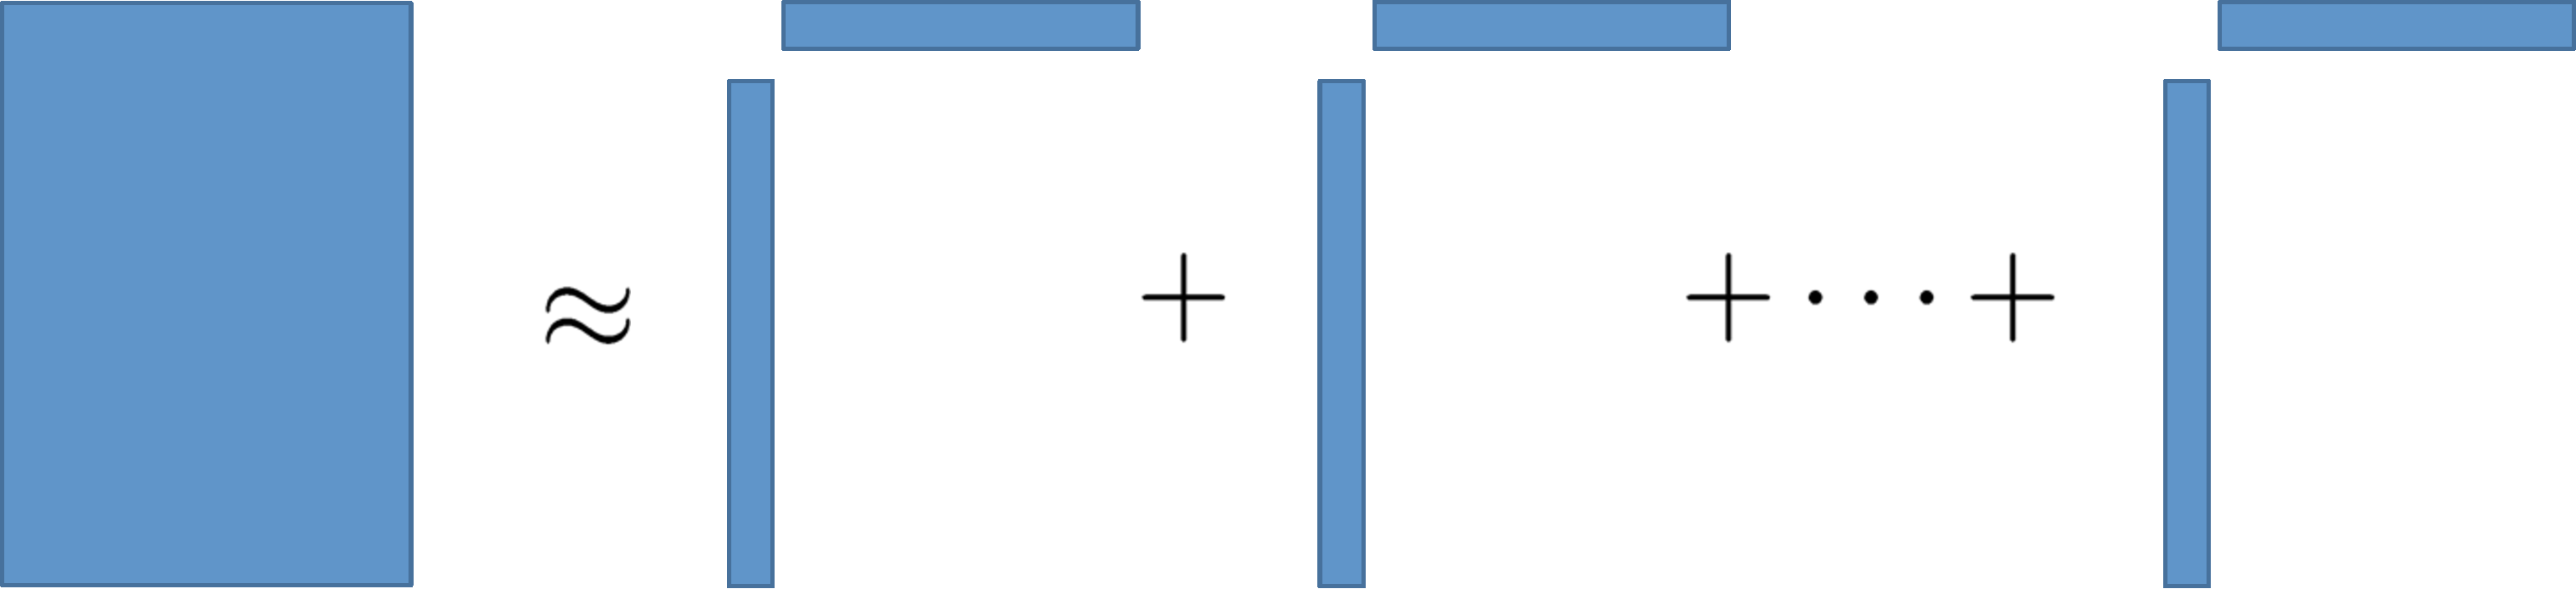
\includegraphics{matrix-LR-SOP}}
\end{center}
\vfill
Tensor: \quad $\displaystyle \T{X}\approx \sum_{r=1}^R (\lambda_r \MC{U}{r})\circ\MC{V}{r}\circ\MC{W}{r}$
\begin{center}
\scalebox{.15}{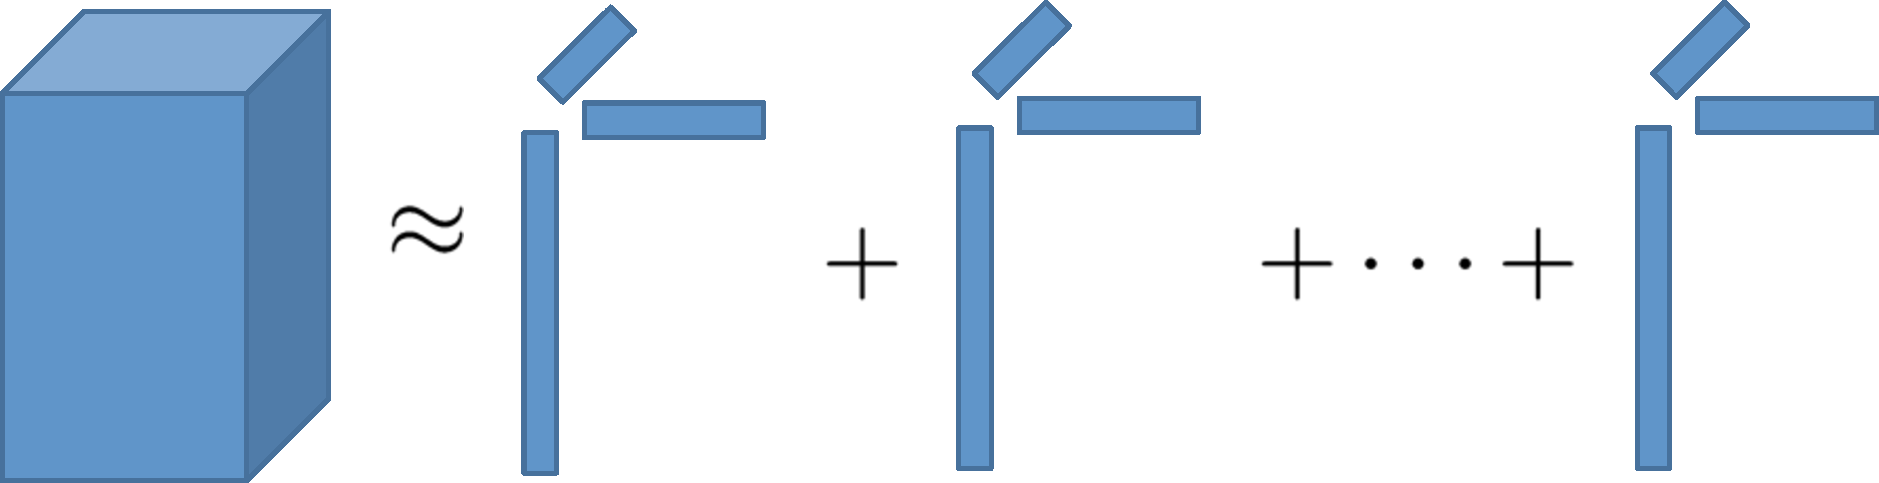
\includegraphics{tensor-LR-SOP}}
\end{center}
\vfill
\begin{itemize}
\item This is known as the CANDECOMP or PARAFAC or canonical polyadic or \textbf{CP decomposition}. It approximate tensors as sum of outer products or rank-1 tensors.
\item NNCP imposes \textbf{non-negativity} constraints on the factor matrices to aid interpretability.
\end{itemize}
\end{frame}

%\begin{frame}
%\frametitle{NNCP Decomposition}
%\begin{itemize} 
%\item NNCP imposes non-negativity constraints on each of the factor matrices.
%\begin{align*}
%\T{X}\approx \sum_{r=1}^R &(\lambda_r \MC{U}{r})\circ\MC{V}{r}\circ\MC{W}{r} \\
%\textnormal{subject to} \\
%\MC{u}{r} &\geq \V{0} \\
%\MC{v}{r} &\geq \V{0} \\
%\MC{w}{r} &\geq \V{0} 
%\end{align*}
%\item NNCP results in a ``parts"-based decomposition with each column $\MC{u}{r}, \MC{v}{r}, \MC{w}{r}$ can only be scaled and added together.
%\item This aids in the interpretability of the factorisation especially if the input data is non-negative.
%\end{itemize}
%\end{frame}

\begin{frame}
\frametitle{Computational Bottlenecks}
\begin{itemize}
\item The MTTKRP is the major bottleneck for NNCP.
$$\Mn{M}{1} = \Mz{X}{1}(\M{W} \Khat \M{V})$$
$$\ME{M}{ir} = \sum_{j=1}^J \sum_{k=1}^K \TE{X}{ijk} \ME{V}{jr} \ME{W}{kr}$$
\item Standard approach is to explicitly matricise the tensor and form the Khatri-Rao product before calling DGEMM.
\item Can we do better? Avoid matricisation of the tensor and full Khatri-Rao products ...
\end{itemize}
\end{frame}

\begin{frame}
\frametitle{Communication Lower Bounds}
\begin{itemize}
\item Following the nested arrays lower bounds~\cite{BKR2017}.
\begin{theorem}
Any parallel MTTKRP algorithm involving a tensor with $I_k=I^{1/N}$ for all $k$ and that evenly distributes one copy of the input and output performs at least
\begin{equation*}
\Omega\left( \left( \frac{NIR}{P} \right)^{\frac{N}{2N-1}} + NR\left(\frac{I}{P}\right)^{1/N} \right)
\end{equation*}
sends and receives.  (Either term can dominate.)
\end{theorem}
\item Key Assumptions: algorithm is not allowed to pre-compute and re-use temporary values.
\item $\Omega\pr{NR\pr{\frac I P}^{1/N}}$ is the most frequently occurring case for relatively small $P$ or $R$.
\end{itemize}
\end{frame}

\begin{frame}
\frametitle{Shared Memory Optimisation - Dimension Trees}
\begin{itemize}
\item Reuse computations across MTTKRPs.
$$\Mn{M}{1}=\underline{\Mz{X}{1}(\Mn{U}{3}}\Khat\Mn{U}{2}) \quad \Mn{M}{2}=\underline{\Mz{X}{2}(\Mn{U}{3}}\Khat\Mn{U}{1})$$
\item Utilise a ``dimension tree" to store and reuse partial products~\cite{PTC13a,LKLHS2017,HBJT18}. 
\begin{center}
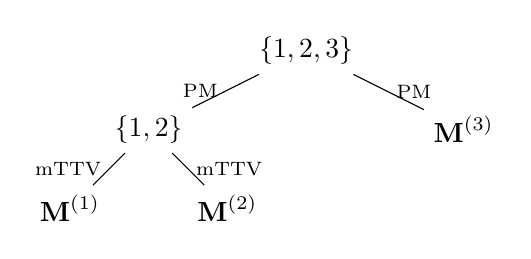
\begin{tikzpicture}

\node (123) at (4,2) {$\{1,2,3\}$};
\node (12) at (2,1) {$\{1,2\}$};
\node (3) at (6,1) {$\Mn{M}{3}$};
\node (1) at (1,0) {$\Mn{M}{1}$};
\node (2) at (3,0) {$\Mn{M}{2}$};

\scriptsize
\path[draw] (123) edge [left,align=right] node {PM} (12);
\path[draw] (123) edge [right,align=left] node {PM} (3);
\path[draw] (12) edge [left,align=right] node {mTTV} (1);
\path[draw] (12) edge [right,align=left] node {mTTV} (2);
\normalsize

\end{tikzpicture}
\end{center}
\item PM = partial MTTKRP 
\item mTTV = multi-Tensor-Times-Vector
\end{itemize}
\end{frame}

\begin{frame}
\frametitle{Distributed Memory Optimisation - Communication Avoiding}

\begin{columns}

\begin{column}{.6\textwidth}

\newcommand{\procdim}{3}
\newcommand{\proc}{\draw[black,shift={(-.5,-.5)}] (0,0) grid (\procdim,\procdim);}
\newcommand{\highlight}{gray!75}
\newcommand{\commhighlight}{gray!25}

\begin{center}
\begin{tikzpicture}[x={(-0.5cm,-0.4cm)}, y={(1cm,0cm)}, z={(0cm,1cm)},every node/.append style={transform shape}]

% highlight all-gather/reduce-scatter patterns
% 1st slide is proc data (leave highlighting for all slides)
% 2nd slide is all-gather in 1st mode
\only<2>{
% front face
\begin{scope}[canvas is yz plane at x=.5]
	% highlight front face of proc comm
	\draw[fill=\commhighlight,shift={(-.5,-.5)}] (0,0) rectangle (3,1);
	% highlight block of 1st factor matrix
	\draw[fill=\commhighlight,shift={(-1,.5)},xscale=.5] (0,0) rectangle (-1,-1);
\end{scope}
% right face
\begin{scope}[canvas is zx plane at y=(\procdim-.5),rotate=-90]
	% highlight right face of proc comm
	\draw[fill=\commhighlight,shift={(-.5,-.5)}] (0,0) rectangle (3,1);
\end{scope}
% top face
\begin{scope}[canvas is yx plane at z=.5,yscale=-1,rotate=0]
	% highlight top face of proc comm
	\draw[fill=\commhighlight,shift={(-.5,-.5)}] (0,0) rectangle (3,3);
\end{scope}
}
% 3rd slide is all-gather in 3rd mode
\only<3>{
% front face
\begin{scope}[canvas is yz plane at x=.5]
	% highlight front face of proc comm
	\draw[fill=\commhighlight,shift={(-.5,.5)}] (0,0) rectangle (3,-3);
	% highlight block of 1st factor matrix now owned by processor
	\draw[fill=\highlight,shift={(-1,.5)},xscale=.5] (0,0) rectangle (-1,-1);
\end{scope}
% right face
\begin{scope}[canvas is zx plane at y=(\procdim-.5),rotate=-90]
	% highlight right face of proc comm
	\draw[fill=\commhighlight,shift={(-.5,.5)}] (0,0) rectangle (1,-3);
	% highlight block of 3rd factor matrix
	\draw[fill=\commhighlight,yscale=.5,shift={(-.5,-6)}] (0,0) rectangle (1,-1);
\end{scope}
% top face
\begin{scope}[canvas is yx plane at z=.5,yscale=-1,rotate=0]
	% highlight top face of proc comm
	\draw[fill=\commhighlight,shift={(-.5,-.5)}] (0,0) rectangle (3,1);
\end{scope}
}
% 4th and 5th slides are local computation
\only<4-5>{
% front face
\begin{scope}[canvas is yz plane at x=.5]
	% highlight block of 1st factor matrix now owned by processor
	\draw[fill=\highlight,shift={(-1,.5)},xscale=.5] (0,0) rectangle (-1,-1);
\end{scope}
% right face
\begin{scope}[canvas is zx plane at y=(\procdim-.5),rotate=-90]
	% highlight block of 3rd factor matrix now owned by processor
	\draw[fill=\highlight,yscale=.5,shift={(-.5,-6)}] (0,0) rectangle (1,-1);
\end{scope}
}
\only<5>{
% front face
\begin{scope}[canvas is yz plane at x=.5]
	% highlight block of 2nd factor matrix contribution computed by processor
	\draw[fill=\highlight,shift={(1.5,-3)},yscale=.5] (0,0) rectangle (1,-1);
\end{scope}
}
% 6th slide is reduce-scatter in 2nd mode
\only<6>{
% front face
\begin{scope}[canvas is yz plane at x=.5]
	% highlight front face of proc comm
	\draw[fill=\commhighlight,shift={(1.5,.5)}] (0,0) rectangle (1,-3);
	% highlight block of 2nd factor matrix involved in reduce scatter
	\draw[fill=\commhighlight,shift={(1.5,-3)},yscale=.5] (0,0) rectangle (1,-1);
	% highlight block of 2nd factor matrix of computed output
	\draw[fill=\highlight,shift={(1.5,-3)},yscale=.5] (0,0) rectangle (1/9,-1);
	% highlight block of 1st factor matrix now owned by processor
	\draw[fill=\highlight,shift={(-1,.5)},xscale=.5] (0,0) rectangle (-1,-1);
\end{scope}
% right face
\begin{scope}[canvas is zx plane at y=(\procdim-.5),rotate=-90]
	% highlight right face of proc comm
	\draw[fill=\commhighlight,shift={(-.5,.5)}] (0,0) rectangle (3,-3);
	% highlight block of 3rd factor matrix now owned by processor
	\draw[fill=\highlight,yscale=.5,shift={(-.5,-6)}] (0,0) rectangle (1,-1);
\end{scope}
% top face
\begin{scope}[canvas is yx plane at z=.5,yscale=-1,rotate=0]
	% highlight top face of proc comm
	\draw[fill=\commhighlight,shift={(1.5,-.5)}] (0,0) rectangle (1,3);
\end{scope}
}
\only<7>{
% front face
\begin{scope}[canvas is yz plane at x=.5]
	% highlight block of 2nd factor matrix of computed output
	\draw[fill=\highlight,shift={(1.5,-3)},yscale=.5] (0,0) rectangle (1/9,-1);
\end{scope}
}

% highlight one processor's data
% front face
\begin{scope}[canvas is yz plane at x=.5,shift={(1.5,-1.5)}]
	% highlight front face of tensor block
	\draw[fill=\highlight,shift={(0,1)}] (0,0) rectangle (1,1);
	% highlight block of 1st factor matrix
	\draw[fill=\highlight,shift={(-2.5,2-1/3)},xscale=.5] (0,0) rectangle (-1,-1/9);
	% highlight block of 2nd factor matrix
	\draw[shift={(0,-1.5)},yscale=.5] (0,0) rectangle (1/9,-1);
\end{scope}
% right face
\begin{scope}[canvas is zx plane at y=(\procdim-.5),rotate=-90,shift={(-.5,-3)}]
	% highlight front face of tensor block
	\draw[fill=\highlight,shift={(0,2.5)}] (0,0) rectangle (1,1);
	% highlight block of 3rd factor matrix
	\draw[fill=\highlight,yscale=.5] (0,0) rectangle (1/9,-1);
\end{scope}
% top face
\begin{scope}[canvas is yx plane at z=.5,yscale=-1,rotate=0]
	% highlight front face of tensor block
	\draw[fill=\highlight,shift={(1.5,-.5)}] (0,0) rectangle (1,1);
\end{scope}

% draw tensor
% front face
\begin{scope}[canvas is yz plane at x=.5,rotate=-90]
	\proc
\end{scope}
% top face
\begin{scope}[canvas is yx plane at z=.5,yscale=-1,rotate=0]
	\proc
\end{scope}
% right face
\begin{scope}[canvas is zx plane at y=(\procdim-.5),rotate=180]
	\proc
\end{scope}

% draw factor matrices
% front face
\begin{scope}[canvas is yz plane at x=.5,shift={(1.5,-.5)}]
	% draw 1st factor matrix
	\draw[shift={(-2.5,0)},xscale=.5] (0,-2) grid (-1,1);
	\node[draw=none] at (-3.5,-.5) {$\Mn{U}{1}$};
	% draw 2nd factor matrix
	\draw[shift={(0,-2.5)},yscale=.5] (-2,0) grid (1,-1);
	\node[draw=none] at (-.5,-3.5) {$\Mn{M}{2}$};
\end{scope}
% right face
\begin{scope}[canvas is zx plane at y=(\procdim-.5),rotate=-90,shift={(1.5,-.5)}]
	% draw 3rd factor matrix
	\draw[shift={(0,-2.5)},yscale=.5] (-2,0) grid (1,-1);
	\node[draw=none] at (-.5,-3.5) {$\Mn{U}{3}$};
\end{scope}


\end{tikzpicture}
\end{center}

\end{column}
\begin{column}{.45\textwidth}

\footnotesize
Each processor
\begin{enumerate}
	\item Starts with one subtensor and subset of rows of each input factor matrix
	\uncover<2->{\item All-Gathers all the rows needed from $\Mn{U}{1}$}
	\uncover<3->{\item All-Gathers all the rows needed from $\Mn{U}{3}$}
	\uncover<4->{\item Computes its contribution to rows of $\Mn{M}{2}$ (local MTTKRP)}
	\uncover<6->{\item Reduce-Scatters to compute and distribute $\Mn{M}{2}$ evenly}
	\uncover<7->{\item Solve local NLS problem using $\Mn{M}{2}$ and $\Mn{U}{2}$}
\end{enumerate}

\end{column}

\end{columns}

\end{frame}

\begin{frame}
\frametitle{Performance Plots - Strong Scaling}
\begin{figure}
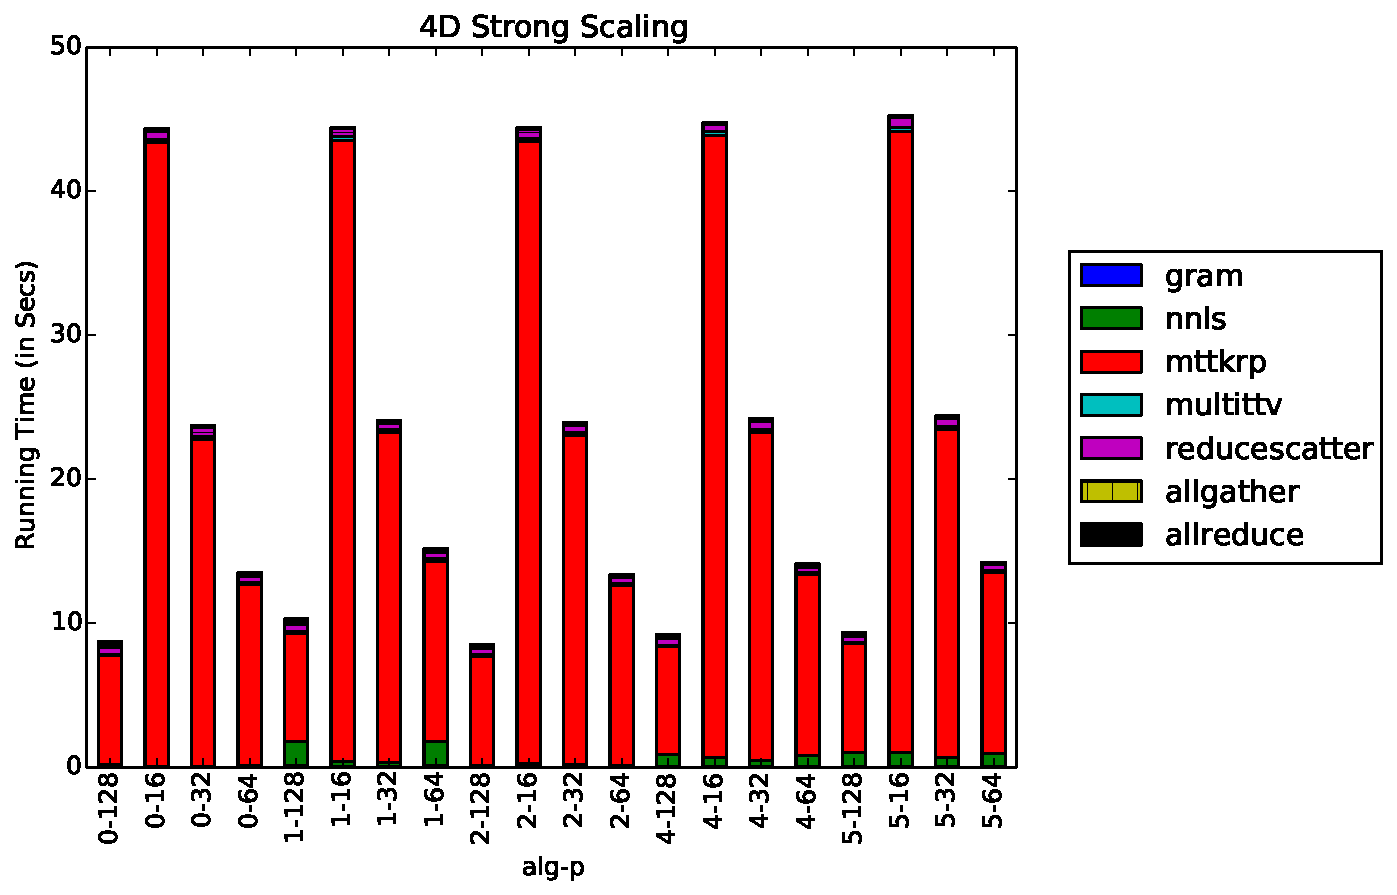
\includegraphics[width=0.7\textwidth]{strsca4d}
\caption{Strong Scaling on synthetic tensor of dimensions $256 \times 256 \times 256 \times 256$ on 8, 16, 32, 64 and 128 nodes of Titan}
\end{figure}
\begin{center}
Can achieve \textbf{nearly linear} scaling since NNCP is compute bound.
\end{center}
\end{frame}

\begin{frame}
\frametitle{Performance Plots - CPU vs GPU}
\begin{columns}[onlytextwidth]
\begin{column}{.5\textwidth}
\begin{figure}
  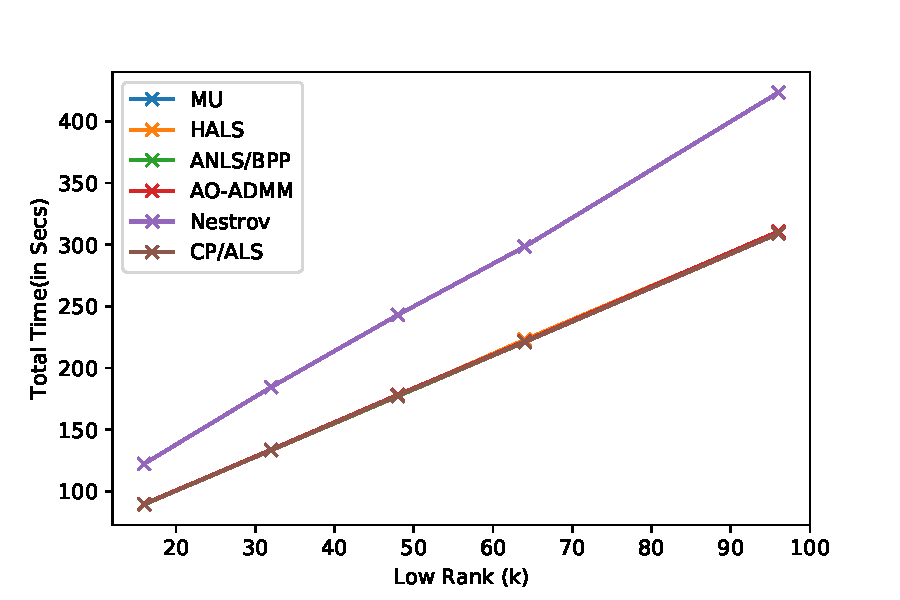
\includegraphics[width=\textwidth]{cpuvsgpulr810}
  \caption{CPU}
\end{figure}
\end{column}
\hfill
\begin{column}{.5\textwidth}
\begin{figure}
  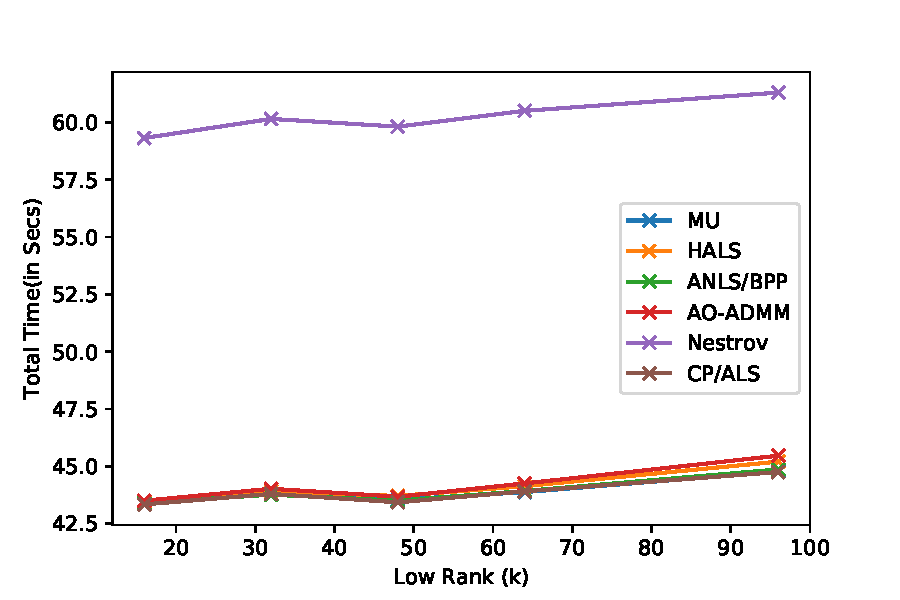
\includegraphics[width=\textwidth]{cpuvsgpulr811}
  \caption{GPU}
\end{figure}
\end{column}
\end{columns}
\begin{center}
\footnotesize{4D synthetic tensor of dimensions $384 \times 384 \times 384 \times 384$ on 81 Titan nodes as a $3 \times 3 \times 3 \times 3$ grid with varying low rank.} 
\end{center}
\begin{center}
Offloading DGEMM calls to GPU can provide \textbf{7X speedup}.
\end{center}
\end{frame}

\begin{frame}
\frametitle{Compiler Challenges and Extensions to the Sparse Setting}
\begin{enumerate}
\item Dimension Tree ordering.
	\begin{itemize}
	\item Combinatorial explosion for sparse case (contrasted with the single split choice for the dense case).
	\item Sparse case involves growth in intermediate values.
	\end{itemize}
\item Communication Pattern establishment and load balancing.
	\begin{itemize}
	\item Automatic communicator setup given a processor grid and tensor operation.
	\item Automatic data distribution using the communication-avoiding loop optimisation~\cite{knight2015communication, DR16arxiv}.
	\end{itemize}
\item Block Parallelism in Least Squares Solvers.
	\begin{itemize}
	\item Active Set orderings can be grouped in an embarrassingly parallel call.
	\item Sparse case with masking matrix has a similar RHS pattern.
	\end{itemize}
\item Binary Bloat
	\begin{itemize}
	\item Separate binaries for GPU/CPU and Sparse/Dense.
	\end{itemize}
\end{enumerate}
\end{frame}

%\againframe{summary}
\begin{frame}[label=summary]
\frametitle{Summary}
\begin{itemize}
\item PLANC is an open source, scalable and flexible software package to compute Non-negative Tensor Factorisation.
\item Implements state of the art communication avoiding algorithm for matricised-tensor times Khatri-Rao product (MTTKRP).
\item Popular optimisation methods like Block Principal Pivoting, Alternating Direction Method of Multipliers, first order Nesterov methods etc. for Non-negative Least Squares are included. 
\item NTF is an important contributor towards explainable AI with a wide range of applications like spectral unmixing, scientific visualization, healthcare analytics, topic modelling etc.
\item Coming soon as a miniapp on OLCF machines. \href{https://github.com/ramkikannan/planc/}{https://github.com/ramkikannan/planc}.
\end{itemize}
\end{frame}

\begin{frame}[allowframebreaks]
\frametitle{References}
\tiny
\bibliographystyle{alpha}
\bibliography{slides}
\normalsize
\end{frame}

\appendix


\begin{frame}
\frametitle{NNCP Algorithm}
\begin{itemize}
\item For given rank $R$ we formulate NNCP as the following optimisation problem,
\begin{align*}
\underset{\M{U},\M{V},\M{W} \geq \M{0}}{\min}\norm{\T{X}-\sum_{r=1}^R \lambda_r\MC{U}{r}\circ\MC{V}{r}\circ\MC{W}{r}}
\end{align*}
\item Non-linear and non-convex problem.
\item Solve via Alternating Non-negative Least Squares in an iterative manner using Block Coordinate Descent.
\end{itemize}
\end{frame}

\begin{frame}
\frametitle{Alternating Non-negative Least Squares (ANLS)}
\begin{itemize}
\item Fixing all factor matrices but one results in a linear NLS problem,
\begin{align*}
&\underset{\M{U} \geq \M{0}}{\min}\norm{\T{X}-\sum_{r=1}^R \MC{U}{r}\circ\MC[\hat]{V}{r}\circ{\MC[\hat]{W}{r}}} \\
&\textnormal{or equivalently,}\\
&\underset{\M{U} \geq \M{0}}{\min} \norm{\Mz{X}{1} -\M{U}(\M[\hat]{W} \Khat \M[\hat]{V})^\Tra}_F
\end{align*}
\item $\Khat$ is the Khatri-Rao product (column-wise Kronecker Product) of the factor matrices.
\item Utilising the identity $(\M{A}\Khat\M{B})^\Tra(\M{A}\Khat\M{B}) = \M{A}^\Tra\M{A} \Hada \M{B}^\Tra\M{B}$, we can cast the above problem as NLS solves via normal equations.
$$\underset{\M{U} \geq \M{0}}{\min} \norm{\Mz{X}{1}(\M[\hat]{W} \Khat \M[\hat]{V}) -\M{U}\pr{\M[\hat]{W}^\Tra\M[\hat]{W} \Hada \M[\hat]{V}^\Tra\M[\hat]{V}}}_F$$
where $\Hada$ is the Hadamard Product.
\end{itemize}
\end{frame}

\end{document}